\documentclass[a4paper,10pt]{article}

\usepackage{graphicx}
\usepackage[utf8]{inputenc}
\usepackage[T1]{fontenc}
\usepackage{wrapfig}

\usepackage{hyperref}
\setlength{\parindent}{10pt}
\setlength{\parskip}{1.5mm}
\usepackage{geometry}
\geometry{margin=1.25cm}
\addtolength{\textheight}{-1.5cm}
\setlength{\headheight}{32pt}

\usepackage{amsfonts, amstext, color,
	ifthen, fancybox, multirow, fancyhdr, pgf, tikz,%
	colortbl, array, tabularx
}

\definecolor{bgcode}{rgb}{0.95,0.95,0.95}

\usepackage{url}

\usepackage[french]{babel}
\selectlanguage{french}

%partie concernant la gestion des entêtes
\usepackage{fancyhdr}
\pagestyle{fancy}
\usepackage{lastpage}
\renewcommand\headrulewidth{1pt}
\fancyhead[L]{Interface Homme-Machine Unity}
\fancyhead[R]{Université de Poitiers}
\renewcommand\footrulewidth{1pt}
\fancyfoot[L]{Département d'Informatique}
\fancyfoot[C]{\textbf{\thepage/\pageref{LastPage}}}
\fancyfoot[R]{année 2022-2023}
%fin

\usepackage{enumitem}

\usepackage{listings}

\usepackage{version}
\usepackage{tcolorbox}

\newcounter{Exercice}
\newcommand{\Exercice}[1]{\refstepcounter{Exercice}%
	\ \vspace{0mm} \\ \hspace{0.8cm}%
	\noindent \hspace*{0.5cm} {\bf Question \theExercice :} #1 \vspace{-13mm} \\ %
	\subparagraph*{}%
}

\lstset{language=Caml,basicstyle=\normalsize\tt,keywordstyle=\ttfamily\bfseries\underbar,%
	commentstyle=\normalsize, extendedchars=true, fontadjust=true, columns = flexible, flexiblecolumns=true,
	linewidth=.975\linewidth, backgroundcolor=\color{bgcode}, frame=tlrb, xleftmargin=1cm}

\lstnewenvironment{ocamlcode}
{\lstset{language=Caml,basicstyle=\normalsize\tt,keywordstyle=\ttfamily\bfseries\underbar,%
		commentstyle=\normalsize, extendedchars=true, fontadjust=true, columns = flexible, flexiblecolumns=true,
		linewidth=.975\linewidth, backgroundcolor=\color{bgcode}, frame=tlrb, xleftmargin=1cm,
		literate={à}{{\`a}}1 {è}{{\`e}}1 {é}{{\'e}}1 {ê}{{\^e}}1,
	}}%, framexleftmargin=5mm,frame=box}}
{}

\lstnewenvironment{fsharp}
{\lstset{language=Caml,basicstyle=\normalsize\tt,keywordstyle=\ttfamily\bfseries\underbar,%
		commentstyle=\normalsize, extendedchars=true, fontadjust=true, columns = flexible, flexiblecolumns=true,
		linewidth=.975\linewidth, backgroundcolor=\color{bgcode}, frame=tlrb, xleftmargin=1cm,
		literate={à}{{\`a}}1 {è}{{\`e}}1 {é}{{\'e}}1 {ê}{{\^e}}1 {ç}{{\c c}}1,
}}%, framexleftmargin=5mm,frame=box}}
{}

\lstnewenvironment{javasansbord}
{\lstset{language=Java,basicstyle=\normalsize\tt,keywordstyle=\ttfamily\bfseries\underbar,%
		commentstyle=\normalsize, extendedchars=true, fontadjust=true, columns = flexible, flexiblecolumns=true,
		linewidth=.975\linewidth,frame=,backgroundcolor=,xleftmargin=0cm,
		literate={à}{{\`a}}1 {è}{{\`e}}1 {é}{{\'e}}1 {ê}{{\^e}}1 {ç}{{\c c}}1,
}}%, framexleftmargin=5mm,frame=box}}
{}

\lstnewenvironment{java}
{\lstset{language=Java,basicstyle=\normalsize\tt,keywordstyle=\ttfamily\bfseries\underbar,%
		commentstyle=\normalsize, extendedchars=true, fontadjust=true, columns = flexible, flexiblecolumns=true,
		linewidth=.975\linewidth, backgroundcolor=\color{bgcode}, frame=tlrb, xleftmargin=1cm,
		literate={à}{{\`a}}1 {è}{{\`e}}1 {é}{{\'e}}1 {ê}{{\^e}}1 {ç}{{\c c}}1,
}}%, framexleftmargin=5mm,frame=box}}
{}

\newboolean{versionenseignant}
%%%%%%%%%%%%%%%%%%%%%%%%%%%%%%%%%%%%%%%%%%%%%%%%%%%%%%%%%%%%%%%%%%%%%%%%%%%%%%%%%%%%%%%%%%%%%%%%%%%%%%%%
%__     __            _
%\ \   / /__ _ __ ___(_) ___  _ __
% \ \ / / _ \ '__/ __| |/ _ \| '_ \
%  \ V /  __/ |  \__ \ | (_) | | | |
%   \_/ \___|_|  |___/_|\___/|_| |_|
% _____                _                         _
%| ____|_ __  ___  ___(_) __ _ _ __   __ _ _ __ | |_
%|  _| | '_ \/ __|/ _ \ |/ _` | '_ \ / _` | '_ \| __|
%| |___| | | \__ \  __/ | (_| | | | | (_| | | | | |_
%|_____|_| |_|___/\___|_|\__, |_| |_|\__,_|_| |_|\__|
%                        |___/ 
%% modifiez le booleen ci-dessous pour generer la version enseignant ou etudiant
%% ===> true = version enseignant
%% ===> false = version etudiant
\setboolean{versionenseignant}{false}
%%%%%%%%%%%%%%%%%%%%%%%%%%%%%%%%%%%%%%%%%%%%%%%%%%%%%%%%%%%%%%%%%%%%%%%%%%%%%%%%%%%%%%%%%%%%%%%%%%%%%%%%
% \includeversion{ensnote}
%\excludeversion{ensnote}
\ifthenelse{\boolean{versionenseignant}}{\includeversion{ensnote}}{\excludeversion{ensnote}}

\tcbuselibrary{breakable}


\newenvironment{solution}%
{\begin{tcolorbox}[breakable,colback=red!5!white,colframe=red!75!black,title=Solution]}%
{\end{tcolorbox}}

%\tcblower

\newenvironment{info}%
{\begin{tcolorbox}[breakable,colback=green!5!white,colframe=green!75!black,title=Information]}%
{\end{tcolorbox}}


\newenvironment{attention}%
{\begin{tcolorbox}[breakable,colback=green!25!white,colframe=red!55!black,title=Attention]}%
{\end{tcolorbox}}


\newenvironment{boxcode}%
{\begin{tcolorbox}[breakable,colback=gray!5!white,colframe=black]}%
	{\end{tcolorbox}}
	
	
\begin{document}
	


\title{\vspace*{-1cm}Réalisation d'un système solaire}
\author{\vspace*{-1.5cm}Interface Homme-Machine: Unity
\begin{ensnote}
	(Version enseignant)
\end{ensnote}
}
\date{\vspace*{-1.5cm}version 1}
\maketitle
\thispagestyle{fancy}

Voici les objectifs de ce sujet:
\begin{itemize}
	\item Comprendre l'IDE \texttt{Unity}.
	\item Création d'un projet.
	\item Placez des objets dans l'environnement.
	\item Comprendre la hiérarchie pour différencier transformation locale et globale.
	\item Comprendre le canevas 2D.
	\item Manipuler des widgets classiques.
	\item Exploiter les événements pour ajouter des interactions.
	\item Réalisation de scripts simple pour l'animation.
\end{itemize}


%\begin{attention}
%	Le sujet ce fait en deux étapes. Avec une proposition notée de votre interface au bout de 2h (si vous avez fini avant la \textit{deadline} rien ne vous empêche de continuer)!
%	
%	N'oubliez pas d'utiliser les bons réflexes de tout développeur:
%	\begin{itemize}
%		\item Le système de log très bien fait sous Android
%		\item Le mode débogue qui vous permet de voir les valeurs des variables pendant 
%	\end{itemize}
%\end{attention}

\section*{Description générale de l'application}

Dans ce TP, nous allons modéliser un système solaire qui n'est pas réaliste physiquement. Pour cela, vous devez réaliser en vous inspirant ce qui a été fait en cours en utilisant la hiérarchie, un système solaire composé des éléments suivants:
\begin{itemize}
	\item Soleil qui est au centre de notre animation.
	\item Deux planètes (disons Terre et Mars) qui tourne autour du soleil.
	\item Des lunes pour chaque planète. Pour information, la Terre possède une lune et Mars possède 2 lunes (nommées Phobos et Deimos). 
\end{itemize}


\begin{center}
	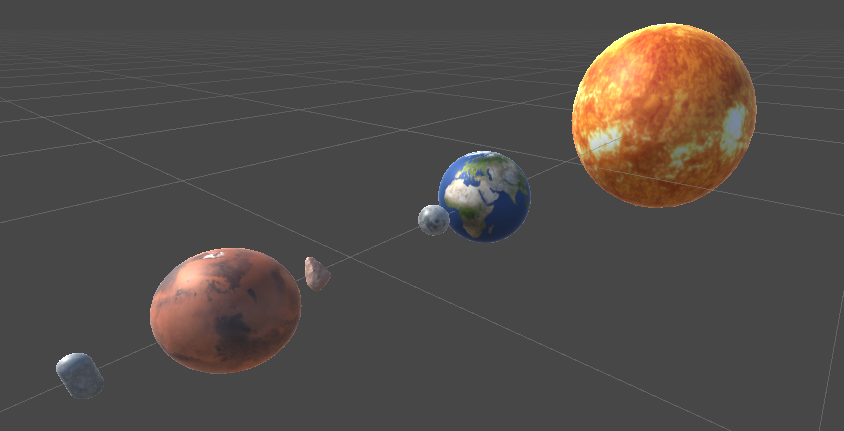
\includegraphics[width=0.7\linewidth]{rc/solarsystem_ez}
\end{center}

L'objectif ici est de réalisez des manipulations d'Unity, vous pouvez/devez expérimenter les points suivants:
\begin{enumerate}
	\item Utilisez la forme primitive Capsule pour Deimos.
	\item Utilisez un maillage produit avec vos mains sous Blender ou via un objet quelconque trouvé sur l'Internet pour remplacer Phobos.
	\item Mettez une texture sur les objets (pas forcément celle des planètes, mais ce que vous voulez).
	\item Modifiez la skybox de votre caméra (plusieurs possibilités, mais utilisez bien la documentation et vos intuitions pour le faire, sans chercher en premier lieu une solution sur le net).
	\item Placez les objets de manière hiérarchique pour obtenir les transformations de leur parent.
\end{enumerate}




\section{Premier script pour animer tout ça}

Je vous propose de réaliser le fameux script JeTourne.cs du cours, qui se contente d'appeler la rotation autour du soleil. Chercher dans la documentation Unity, le rôle de la fonction \texttt{FixedUpdate}. Modifiez votre programme pour l'utiliser en conséquence comme dans le cours. Nous ferons en particulier les variables suivantes sans les liées à des boutons ou autre widget:
\begin{itemize}
	\item Mettez dans votre script une variable booléenne qui détermine si l'objet en question tourne ou non
	\item Mettez la vitesse de rotation de votre objet en guise de paramètre.
	\item Surcharger les fonctions intéressantes du cycle de vie de votre objet pour en faire un affichage dans la console. 
\end{itemize}

\section{Interaction pour le contrôle du système solaire}

Réalisez l'interface proposée ci-dessous pour le soleil:
\begin{center}
	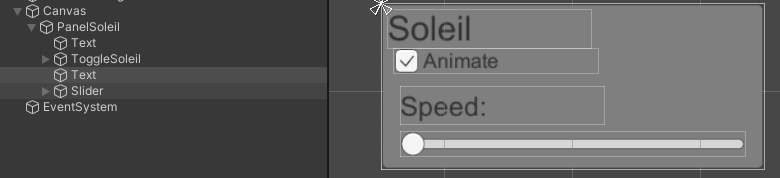
\includegraphics[width=0.7\linewidth]{rc/ui_control_sun_planet}
\end{center}

Ensuite sur ce même modèle, réalisez l'interface pour la Terre et Mars uniquement. Maintenant que vous avez une jolie interface, nous allons réalisez la connexion au écouteur d'événement des boutons d'animation pour contrôler si oui ou non la rotation de l'astre associé est actif ou non. En bref, il vous est demandé de réaliser une fonction, qui détecte les changements de valeur de la checkbox pour en activer/désactiver l'animation selon la valeur du booléen. 
Pour Le slider, nous considérons qu'il pourra prendre des valeurs de 0 à 100 et qui contrôlera la vitesse de rotation de l'objet associé.


\section{Placement de caméra}

Lisez la page du guide suivant: \url{https://docs.unity3d.com/Manual/MultipleCameras.html}. Elle explique les deux façons de contrôler l'affichage d'une caméra simplement.

Pour mettre en pratique les explications du lien, nous vous proposons d'ajouter une caméra local à la Lune (de la Terre). Ajoutez des widgets à l'interface pour changer de caméra à la volée comme indiquez dans la documentation.

Pour les explications de la seconde partie, on se propose d'ajouter une 3e caméra en vu de haut de notre système solaire. Cette vue devra apparaitre en miniature dans le bord bas gauche de la fenêtre (ou un autre bord si vous préférez).


\section{Pour aller plus loin}

La mécanique céleste mise en place jusqu'à présent est vraiment catastrophique, mais offre un cadre suffisant pour l'apprentissage des mécaniques. Nous vous proposons d'ajouter une comète cyclique (ou autre astre) qui n'est plus sous-fils du Soleil, mais bien un objet quelconques.

Pour pouvoir animer votre comète vous allez devoir lui fournir une équation qui va traduire sa trajectoire pour cela je vous propose de vous inspirez du lien suivant \url{https://fr.wikipedia.org/wiki/Trajectoire_d%27une_com%C3%A8te}
ou d'utiliser l'équation d'un cercle autour du soleil par exemple.

\section{Toujours plus loin}

Si vous avez tout fini, nous pouvons complexifier les traitements en regardant la documentation:
\begin{itemize}
	\item En utilisant la fonction \texttt{LookAt} dans la classe \texttt{Transform}, ajoutez pour chaque interface un bouton \texttt{'Center View'} qui centre la vue de la caméra principale vers l'astre associé.
	\item Modifier votre traitement précédent pour que la caméra tourne doucement vers sa position finale pour éviter de perdre l'utilisateur ou lui donner des nausées. Pour cela, nous utiliserons une interpolation linéaire pour entre le point de vue de départ et le point de vue d'arrivé avec une vitesse constante.
\end{itemize}


\end{document}